%%
%% brf.tex
%% Made by nicuveo <antoine.jp.leblanc@gmail.com>
%%



%%%%%%%%%%%%%%%%%%%%%%%%%%%%%%%%%%%%%%%%%%%%%%%%%%%%%%%%%%%%%%%%%%%%%%%%%%%%
%% Header

\documentclass[17pt]{beamer}

\usepackage[english]{babel}
\usepackage{beamerthemesplit}
\usepackage{graphicx}
\usepackage{colortbl}
\usepackage{floatflt}
\usepackage{xunicode}
\usepackage{wasysym}

\title{Learn You a Brainfuck for Great Good!}
\author{Antoine Leblanc\\\small @nicuveo}
\date{\small{January, 2014}}



%%%%%%%%%%%%%%%%%%%%%%%%%%%%%%%%%%%%%%%%%%%%%%%%%%%%%%%%%%%%%%%%%%%%%%%%%%%%
%% Customization

%%
%% theme.tex
%% Made by nicuveo <antoine.jp.leblanc@gmail.com>
%%


%%%%%%%%%%%%%%%%%%%%%%%%%%%%%%%%%%%%%%%%%%%%%%%%%%%%%%%%%%%%%%%%%%%%%%%%%%%%
%% Base theme

\mode<presentation>{}
\usecolortheme{whale}
\usepackage{fontspec}
\setsansfont[Ligatures=TeX, UprightFont={[*-Regular.otf]}, BoldFont={[*-Bold.otf]}]{YanoneKaffeesatz}
\setmonofont{Inconsolata}



%%%%%%%%%%%%%%%%%%%%%%%%%%%%%%%%%%%%%%%%%%%%%%%%%%%%%%%%%%%%%%%%%%%%%%%%%%%%
%% Colors

% define

\definecolor{my-color-1}{RGB}{121,   2,  87} % primary
\definecolor{my-color-2}{RGB}{250, 132, 216} % lighter
\definecolor{my-color-3}{RGB}{  0,   0,   0} % unknown
\definecolor{my-color-4}{RGB}{  0,   0,   0} % darker

\definecolor{tab-1}{rgb}{0.04,0.34,0.58}
\definecolor{tab-2}{rgb}{0.36,0.56,0.72}
\definecolor{tab-3}{rgb}{0.68,0.78,0.86}


% set

\setbeamercolor{structure}{fg=my-color-1}
\setbeamercolor{alerted text}{fg=my-color-1!56!red}

\setbeamercolor{palette primary}   {fg=white, bg=my-color-1}
\setbeamercolor{palette secondary} {fg=black, bg=my-color-2}
\setbeamercolor{palette tertiary}  {fg=white, bg=my-color-3}
\setbeamercolor{palette quaternary}{fg=white, bg=my-color-4}

\setbeamercolor{page number in head/foot} {fg=black, bg=white}
\setbeamercolor{icon in head/foot} {fg=black, bg=white}

\setbeamercolor*{separation line}{}
\setbeamercolor*{fine separation line}{}



%%%%%%%%%%%%%%%%%%%%%%%%%%%%%%%%%%%%%%%%%%%%%%%%%%%%%%%%%%%%%%%%%%%%%%%%%%%%
%% Templates

\setbeamertemplate{headline}[default]

\defbeamertemplate{footline}{mine}[2]
{
  \leavevmode%
  \hbox
  {%
    \begin{beamercolorbox}[wd=.160\paperwidth,ht=3ex,dp=3ex,center]{icon in head/foot}
      \pgfimage[mask=#2,interpolate=true,height=16pt]{#1}
    \end{beamercolorbox}%

    \hskip .740\paperwidth

    \begin{beamercolorbox}[wd=.100\paperwidth,ht=3ex,dp=3ex,center]{page number in head/foot}
      \usebeamerfont{page number in head/foot}
      \insertframenumber{} / \inserttotalframenumber{}
    \end{beamercolorbox}%
  }%
  \vskip0pt%
}

\newcommand{\setfooterlogo}[2]
{
  \setbeamertemplate{footline}[mine]{#1}{#2}
}

%\pgfdeclaremask{masklogo}{img/logo}
\newcommand\defaultlogo{\setfooterlogo{img/ht}{}}
\defaultlogo

\setbeamersize{text margin left=10pt,text margin right=10pt}



%%%%%%%%%%%%%%%%%%%%%%%%%%%%%%%%%%%%%%%%%%%%%%%%%%%%%%%%%%%%%%%%%%%%%%%%%%%%
%% Fonts

\setbeamerfont{frametitle}{size=\small}
\setbeamerfont{structure}{series=\bfseries}



%%%%%%%%%%%%%%%%%%%%%%%%%%%%%%%%%%%%%%%%%%%%%%%%%%%%%%%%%%%%%%%%%%%%%%%%%%%%
%% Settings

\setbeamertemplate{navigation symbols}{}

\bibliographystyle{apalike}

\mode<all>


\renewcommand{\(}[1]{\begin{columns}[#1]}
\renewcommand{\)}{\end{columns}}
\newcommand{\<}[1]{\begin{column}{#1}}
\renewcommand{\>}{\end{column}}



%%%%%%%%%%%%%%%%%%%%%%%%%%%%%%%%%%%%%%%%%%%%%%%%%%%%%%%%%%%%%%%%%%%%%%%%%%%%
%% Document

\begin{document}



%% Title frame

\begin{frame}[fragile]
  \titlepage
\end{frame}



%% Intro

\begin{frame}
  \frametitle{Esoteric languages}
  \begin{itemize}
  \item Have fun\alt<1>{?}{!}
  \item Mess with your brain\alt<1>{?}{!}
  \item Explore new paradigms\alt<1>{?}{!}
  \end{itemize}
    \pause ~\\
  \begin{center}
  \textbf{...all of the above!}
  \end{center}
\end{frame}



%% Joke

\begin{frame}
  \frametitle<2>{Whitespace}
  \begin{center}
  \includegraphics<2>{img/lol}
  \end{center}
\end{frame}



%% Plan

\begin{frame}
  \frametitle{Today's menu}

  \({c}
    \<{6cm}
      \begin{itemize}
      \item Turing-completeness
      \item Brainfuck
      \item Piet
      \item<2> \textbf{$\Rightarrow$ Great good!}
      \end{itemize}
    \>
    \<{7cm}
     \uncover<2>{
\includegraphics[width=6cm]{img/doge}}
    \>
  \)

\end{frame}



%% Turing machine

\begin{frame}
  \frametitle{Turing machine}
  \begin{itemize}
  \item Infinite ribbon of (finite state) cells
  \item Left / right movement
  \item Choice and action on current cell
  \end{itemize}
  \begin{center}
    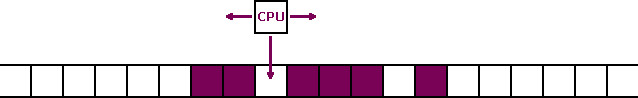
\includegraphics[width=10cm]{img/turing}\\~\\
    Can solve all possible algorithmic computations
  \end{center}
\end{frame}



%% Turing complete

\begin{frame}
  \frametitle{Turing complete languages}
  \begin{itemize}
  \item Simulate any Turing machine
  \item $\Rightarrow$ all possible algorithmic computations
  \pause
  \item $\Rightarrow$ all possible programs!
  \pause
  \item $\Rightarrow$ \structure{...``equivalent'' to all other Turing-complete languages!}
  \end{itemize}
\end{frame}



%% Brainfuck

\begin{frame}
  \frametitle{Brainfuck}
  \begin{center}
    \begin{tabular}{ l c c c }
      Left / right movement & $\Rightarrow$ & < & > \\
      Increment / decrement & $\Rightarrow$ & + & - \\
      Test ``loop'' & $\Rightarrow$ & [ & ] \\
      Byte IO & $\Rightarrow$ & , & .
    \end{tabular}
  \end{center}

  \begin{center}
    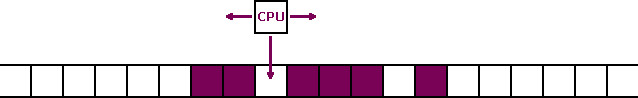
\includegraphics[width=10cm]{img/turing}
    ~\\
    ~\\
    ``Infinite'' buffer of byte cells
  \end{center}
\end{frame}

\begin{frame}
  \frametitle{Brainfuck - Addition}
  \pause
  \begin{center}
    \texttt{~>~[~-~<~+~>~]~<~}
  \end{center}
\end{frame}

\begin{frame}
  \frametitle{Brainfuck - Divmod}
  \pause
  \texttt{\tiny >>>>>>>[-]<<<<<[-]<<[->>+<<]>>>[-]<<<[-]>>[-<<+>>>+<]>[-<+>][-]<<[->>+<<]>>>[-]<<<[-]>>[-<<+>>>+<]>[-<+>][-]<<[->>+<<][-]>[-<+>][-]>[-<+>]>>[-]+<<<<[->>>>[-]<<[-]>[-]<<[->>+<+<]>[-<+>]>[[-]<<->>>[-]+<]<<<]>[[-]>>>[-]+<<<]>>>[>+<<<<[-]<<[->>+<<]>>>[-]<<<[-]>>[-<<+>>>+<]>[-<+>]<[-<<<->>>]<[-]<<[->>+<<]>>>[-]<<<[-]>>[-<<+>>>+<]>[-<+>][-]<<[->>+<<]>>>[-]<<<[-]>>[-<<+>>>+<]>[-<+>][-]<<[->>+<<][-]>[-<+>][-]>[-<+>]>>[-]+<<<<[->>>>[-]<<[-]>[-]<<[->>+<+<]>[-<+>]>[[-]<<->>>[-]+<]<<<]>[[-]>>>[-]+<<<]>>>][-]<<<<<<[->>>>>>+<<<<<<]>>>>>>}
\end{frame}



%% Piet

\begin{frame}
  \frametitle{Piet}
  \begin{itemize}
  \item Image as source
  \item 20 significant colors (18 + B\&W)
  \item Color transition: 17 instructions
  \end{itemize}
  \begin{center}
    
\includegraphics[width=10cm]{img/rainbow}\\~\\
  \end{center}
\end{frame}

\begin{frame}
  \frametitle{Piet!}
  \vspace{-1cm}
  \begin{columns}[t]
    \begin{column}{5cm}
      \begin{center}
        {\footnotesize \alt<1>{?}{Painting}}~\\~\\
        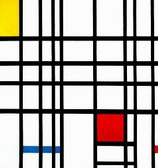
\includegraphics[height=2cm]{img/mondrian}\\~\\
        \uncover<2>{\footnotesize \textbf{Composition with Red, Yellow and Blue} \\ Piet Mondrian}
      \end{center}
    \end{column}
    \begin{column}{5cm}
      \begin{center}
        {\footnotesize \alt<1>{?}{Program}}~\\~\\
        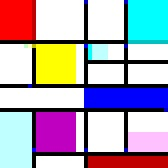
\includegraphics[height=2cm]{img/piet}\\~\\
        \uncover<2>{\footnotesize Prints ``Piet''}
      \end{center}
    \end{column}
  \end{columns}
\end{frame}

\begin{frame}
  \frametitle{Piet!!}
  \vspace{-0.5cm}
  \begin{columns}[t]
    \begin{column}{5cm}
      \begin{center}
        
\includegraphics[width=1.6cm]{img/hw}\\
        {\small Prints ``Hello, world!''}
      \end{center}
    \end{column}
    \begin{column}{5cm}
      \begin{center}
      
\includegraphics[width=1.6cm]{img/hw2}\\
      {\small Prints ``Hello, world!''}
      \end{center}
    \end{column}
  \end{columns}
  \begin{center}
    ~\\~\\
    
\includegraphics[width=2cm]{img/pf}\\
    {\small Prime factor decomposition}
  \end{center}
\end{frame}



%% Both

\begin{frame}
  \frametitle{Why don't we have both?}
  \begin{center}
    
\includegraphics[width=4cm]{img/bf}\\
    {\footnotesize Brainfuck interpreter}\\
    \vspace{0.5cm}
    {\tiny \url{http://www.dangermouse.net/esoteric/piet/samples.html}}
  \end{center}
\end{frame}



%% Others

\begin{frame}[fragile]
  \frametitle{What else?}
  \begin{itemize}
  \item Malbolge
  \end{itemize}
  \begin{center}
    \vspace{-1cm}
    {\tiny \verb;(=<`#9]~6ZY32Vx/4Rs+0No-&Jk)"Fh}|Bcy?`=*z]Kw%oG4UUS0/@-ejc(:'8dc;}
  \end{center}

  \vspace{-0.5cm}

  \begin{itemize}
    \item Unlambda
  \end{itemize}
  \begin{center}
    \vspace{-1cm}
    {\tiny \verb+`r```````````.H.e.l.l.o. .w.o.r.l.di+}
  \end{center}

  \vspace{-0.5cm}

  \begin{itemize}
    \item LOLCODE
  \end{itemize}
  \begin{center}
    \vspace{-1cm}
    {\tiny \verb+HAI; CAN HAS STDIO?; VISIBLE "HAI WORLD!"; KTHXBYE;+}
  \end{center}

  \pause

  \begin{center}
    {\tiny \url{http://esolangs.org/}}
  \end{center}

\end{frame}



%% Great good

\begin{frame}
  \frametitle{Aforementioned great good}
  \begin{itemize}
  \item Impress / frighten your friends!
  \item Draw nice pictures!
  \end{itemize}
  \pause
  \begin{itemize}
  \item Grasp Turing machines!
  \item Stimulate your creativity!
  \item Feed your curiosity!
  \end{itemize}
  \pause
  \begin{itemize}
  \item Give a talk! \smiley
  \end{itemize}
\end{frame}



%% Conclusion

\begin{frame}
  \frametitle{The End}
  \begin{center}
    \textbf{Have fun!}
  \end{center}
\end{frame}



%%%%%%%%%%%%%%%%%%%%%%%%%%%%%%%%%%%%%%%%%%%%%%%%%%%%%%%%%%%%%%%%%%%%%%%%%%%%
%% End

\end{document}
